\documentclass{article}
\setlength{\parskip}{0pt} % esp. entre parrafos
\setlength{\parindent}{20pt} % esp. al inicio de un parrafo
\usepackage{amsmath} % mates
\usepackage{listings}
\usepackage{xcolor}
\usepackage[sort&compress,numbers]{natbib} % referencias
\usepackage{url} % que las URLs se vean lindos
\usepackage[top=10mm,left=20mm,right=20mm,bottom=25mm]{geometry} % \textbf{\textbf{}}margenes
\usepackage{hyperref} % ligas de URLs
\usepackage{graphicx} % poner figuras
\usepackage{caption}
\usepackage{subcaption}
\usepackage[spanish]{babel} % otros idiomas
\hypersetup{
    colorlinks=true,
    linkcolor=blue,
    filecolor=blue,      
    urlcolor=blue,
}
\renewcommand{\lstlistingname}{Código}
\definecolor{codeblack}{rgb}{0,0.6,0}
\definecolor{codegray}{rgb}{0.5,0.5,0.5}
\definecolor{codepurple}{rgb}{0.58,0,0.82}
\definecolor{backcolour}{rgb}{0.95,0.95,0.92}
\lstdefinestyle{mystyle}{
    backgroundcolor=\color{backcolour},   
    commentstyle=\color{codeblack},
    keywordstyle=\color{blue},
    numberstyle=\tiny\color{codegray},
    stringstyle=\color{codeblack},
    basicstyle=\ttfamily\footnotesize,
    breakatwhitespace=false,         
    breaklines=true,                 
    keepspaces=true,                 
    numbers=left,                    
    numbersep=5pt,                  
    showspaces=false,                
    showstringspaces=false,
    showtabs=false,                  
    tabsize=2
}
\lstset{style=mystyle}

\title{"P8" Modelo De Urnas}
\author{NESTOR}
\date {Abril 2022}

\begin{document}

\maketitle

\section{Objetivo}\label{obj}
El objetivo de la práctica consiste sobre fenómenos de coalescencia y fragmentación, donde las partículas se unen para formar cúmulos y estos cúmulos se pueden volver a descomponer en fragmentos menores. Supongamos que cúmulos con $c$ o más partículas son suficientemente grandes para filtrar. Se estudiará el efecto de la tasa $n/k$, usando por lo menos cinco valores distintos para ella, el porcentaje de las partículas que se lograría filtrar por iteración. \cite{elisa1}

\section{Desarrollo}\label{des}
Basando el desarrollo en la \href{https://github.com/satuelisa/Simulation/blob/master/UrnModel/onlyAggr.py}{codificación} implementado por E. Schaeffer \cite{elisa1} y todas las instrucciones se encuentra en el repositorio \href{https://github.com/NestorZeus/SIMULACION-COMPUTACIONAL-DE-NANOMATERIALES/tree/main/P8}{repositorio} de N. Rodríguez en GitHub.\\

Para comenzar se hace primero generar la función para graficar los cúmulos $n/k$ que van a ser los cúmulos, implementados por E. Schaeffer, como se muestra a continuación en el código.

\begin{lstlisting}[caption=Generamos la función, language=Python]
from random import random
from numpy.random import shuffle
import matplotlib.pyplot as plt
from math import exp, floor, log
import numpy as np
from random import randint
def rotura(x, c, d):
    return 1 / (1 + exp((c - x) / d))
def union(x, c):
    return exp(-x / c)
def romperse(tam, cuantos):
    if tam == 1: # no se puede romper
        return [tam] * cuantos
    res = []
    for cumulo in range(cuantos):
\end{lstlisting}

Posteriormente generaramos los ciclos. Para esta práctica se usará 6 variaciones de las 5 que se propusieron en clase como mínimo, esto para variar $n/k$ que se puedan ver las réplicas, a continuación se muestra el código.

\begin{lstlisting}[caption=Generamos los ciclos para variar $n/k$, label=codigo2, language=Python]
k1=(500,8000,20000)
repeticiones=50
for k in k1:
    n1=((k*10),(k*500))
    contador=0
    for n in n1:
        print("########### k,n:",k,n,"#################")
        promedio=[]
\end{lstlisting}

Se realiza el valor $c$ de los cúmulos, a continuación se muestra la siguiente instrucción:
\begin{lstlisting}[caption=Generamos valor $c$, label=codigo2, language=Python]
c = np.median(cumulos) 
d = np.std(cumulos) 
duracion = 50
digitos = floor(log(duracion, 10)) + 1
part_porc=[]
for paso in range(duracion):
    assert sum(cumulos) == n
    assert all([c > 0 for c in cumulos]) 
    (tams, freqs) = np.unique(cumulos, return_counts = True)
    cumulos = []
    assert len(tams) == len(freqs)
\end{lstlisting}

Se realiza un ciclo for porcentaje para los cúmulos que se lograría filtrar por iteración para las partículas como se muestra la siguiente instrucción:

\begin{lstlisting}[caption=Ciclo for para porcentaje de las partículas, label=codigo3, language=Python]
grandes=[]
for s in cumulos:
    if s > c:
        grandes.append(s)
part_porc.append((len(grandes)/len(cumulos))*100)
\end{lstlisting}

Para esto se revisa todos los cumulos una vez que ya se filtraron y si el cumulo es mayor a mi valor crítico, entonces lo voy a guardar en una lista y en este caso son los que se quedaron en el filtro. Para este caso se guarda en un caja bigote como se muestra en el código \ref{codigo3} 

\begin{lstlisting}[caption=Promedio, label=codigo3, language=Python]
promedio.append((sum(part_porc)/len(part_porc)))
        CB.append(promedio)
        ticks.append((str(k),str(n)))
print(len(CB))
print(ticks)
plt.boxplot(CB, [1,2,3,4,5,6])
plt.xlabel('Tasa k/n')
plt.ylabel('Promedios retenidos en filtro (%)')
plt.xticks([1,2,3,4,5,6], ticks,rotation=10)
plt.show()
\end{lstlisting}

\section{Resultados}\label{res}

En la caja bigote nos muestra las combinaciones de las réplicas que se obtiene una cantidad de promedios de porcentaje en el eje $x$ se grafica de la tasa $n/k$ y con en el eje $y$ se grafica los promedios retenidos en el filtro para poder tener el porcentaje, se sacan varios porcentajes ya que se filtraron para poder tener el promedio.

\newpage
\begin{figure}
    \centering
    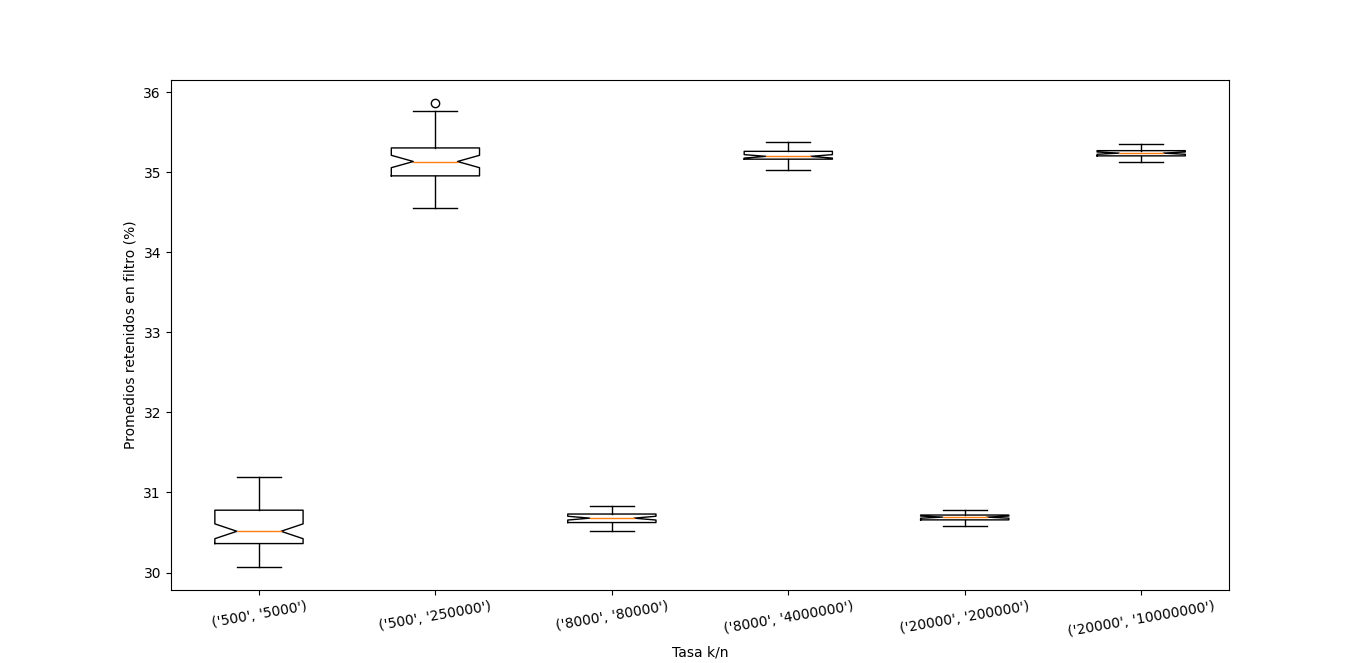
\includegraphics[width=210mm]{Figure_1.png}
    \caption{Diagrama de cúmulos $n/k$.}
    \label{figure}
\end{figure}


\section{Conclusiones}\label{}
Se concluye que los valores, si hacemos la prueba, esto nos da la variación mejor si aumentamos mas la tasa $n/k$ esto para generar mejor el resultado, esto aumenta el promedio de retenidos en el filtro y nos da mejor el comportamiento pero para la tasa de $n$


\newpage
\section{Reto 1 Determinar el filtrado dependiendo del valor $c$}\label{}
En este reto consiste en determinar cómo el momento idóneo de filtrado depende del valor de $c$, esto para saber si todo cambia y como si $c$ ya no se asigna como la mediana inicial sino a un valor menor ó mayor A continuación se muestra en las siguientes instrucciones: 

\begin{lstlisting}[caption=Variación de $c$ en tres diferentes métodos, language=Python]
k = 5000
n = 1000000
repeticiones=40
contador=0
metodos=3 
for met in range(metodos):
    promedio=[]
    for rep in range(repeticiones):
\end{lstlisting}


Para este caso se filtra dependiendo de $c$,
\begin{lstlisting}[caption=Valor filtrado dependiendo de $c$, language=Python]
if contador == 0:
    c = np.median(cumulos)           
elif contador==1:
    c = min(cumulos)# factor arbitrario para suavizar la curva
elif contador==2:
    c = max(cumulos)
\end{lstlisting}


\section{Reto 1 Resultados}\label{}
Para la caja bigote vemos que en el eje $x$, se varía el valor crítico de los cúmulos aquí es con la mediana, el promedio anda de $35.0$ a $35.2$ porciento. Cuando toma el valor mínimo de la lista de cúmulos, el valor mínimo será la rejilla, entonces si un cúmulo es mayor al mínimo se quedará en el filtro, en este caso se tiene un mayor porcentaje que se quede retenidos en el filtro, ya que es el mejor comportamiento. Si se toma el valor máximo son pocos de rejillas aunque no es mejor que la mediana pero se retiene en el filtro.

\begin{figure}
    \centering
    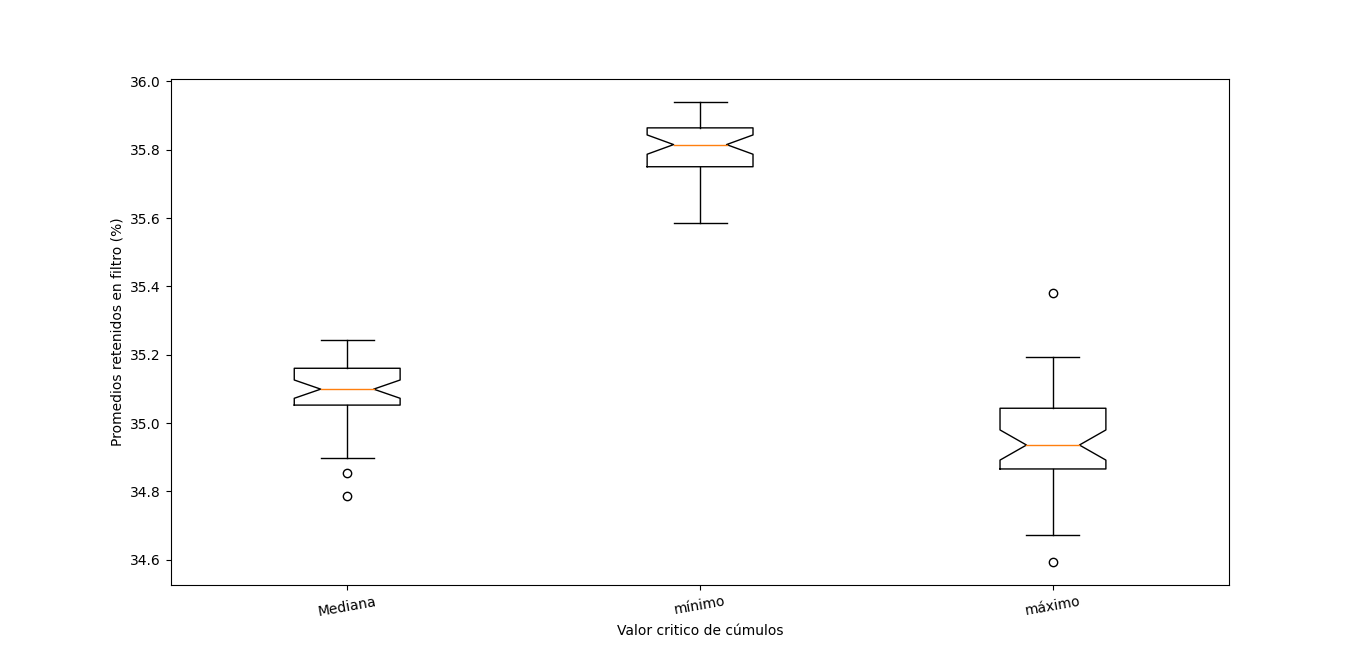
\includegraphics[width=210mm]{R1_box.png}
    \caption{Diagrama bigote dependiendo del valor $c$.}
    \label{figure}
\end{figure}

En las réplicas se muestra que el mínimo, ya que tiene mayor porcentaje, en la réplica máximo si le compite al valor de la mediana pero ya cuando a mayor número de réplicas ya es comparable al de la mediana, en este caso si sea más réplicas tiene un mejor comportamiento y podría ganarle a la mediana a continuación se muestra los siguientes diagramas para el bigote y para las réplicas:

\begin{figure}
    \centering
    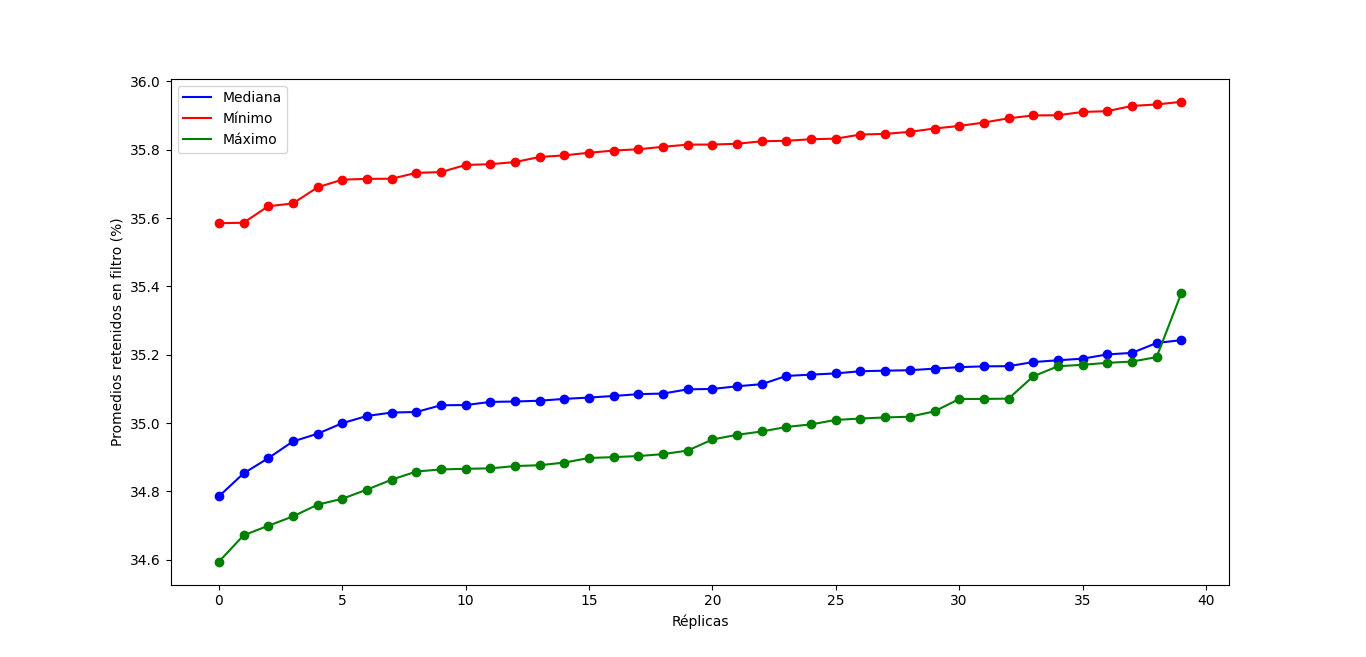
\includegraphics[width=210mm]{R1_plot.png}
    \caption{Diagrama de réplicas dependiendo del valor $c$.}
    \label{figure}
\end{figure}

\newpage

\section{Reto 2 Se estudia el efecto del parámetro suavizante $d$}\label{}
En este reto consiste en el desempeño de filtrado si la meta es recuperar la mayor cantidad posible de partículas en el proceso. ¿En cuál iteración es conveniente realizar el filtrado? Incluye visualizaciones para justificar las conclusiones. A continuación se muestra en las siguientes instrucciones: 

\begin{lstlisting}[caption=Generación de repeticiones, language=Python]
k = 10000
n = 1000000
repeticiones=40
contador=0
metodos=4 
for D in range(metodos):
    promedio=[]
    for rep in range(repeticiones):
\end{lstlisting}

Para este caso la mayor cantidad posible de partículas en el proceso suavizante en $d$.
\begin{lstlisting}[caption=Promedio en el suavizante $d$, language=Python]
if contador == 0:
    d = np.std(cumulos) / 2
elif contador == 1:
    d = np.mean(cumulos)
elif contador==2:
    d = min(cumulos)# factor arbitrario para suavizar la curva
elif contador==3:
    d = max(cumulos)
for paso in range(duracion):
    assert sum(cumulos) == n
    assert all([c > 0 for c in cumulos]) 
    while len(j) > 1: # agregamos los pares formados
        cumulos.append(j.pop(0) + j.pop(0))
    if len(j) > 0: # impar
        cumulos.append(j.pop(0)) # el ultimo no alcanzó pareja
    assert len(j) == 0
    assert sum(cumulos) == n
    assert all([c != 0 for c in cumulos])
    grandes=[]
    for s in cumulos:
        if s > c:
            grandes.append(s)
    cuantos.append(len(grandes))
promedio.append((sum(cuantos)/len(cuantos)))
\end{lstlisting}

\section{Reto 2 Resultados}\label{}
Se muestra como se varía los promedios retenidos en el filtro con los parámetros del suavizante en $d$ de los cúmulos, esto nos ayuda para tener la mayor cantidad de partículas que es el mejor comportamiento. 

\begin{figure}
    \centering
    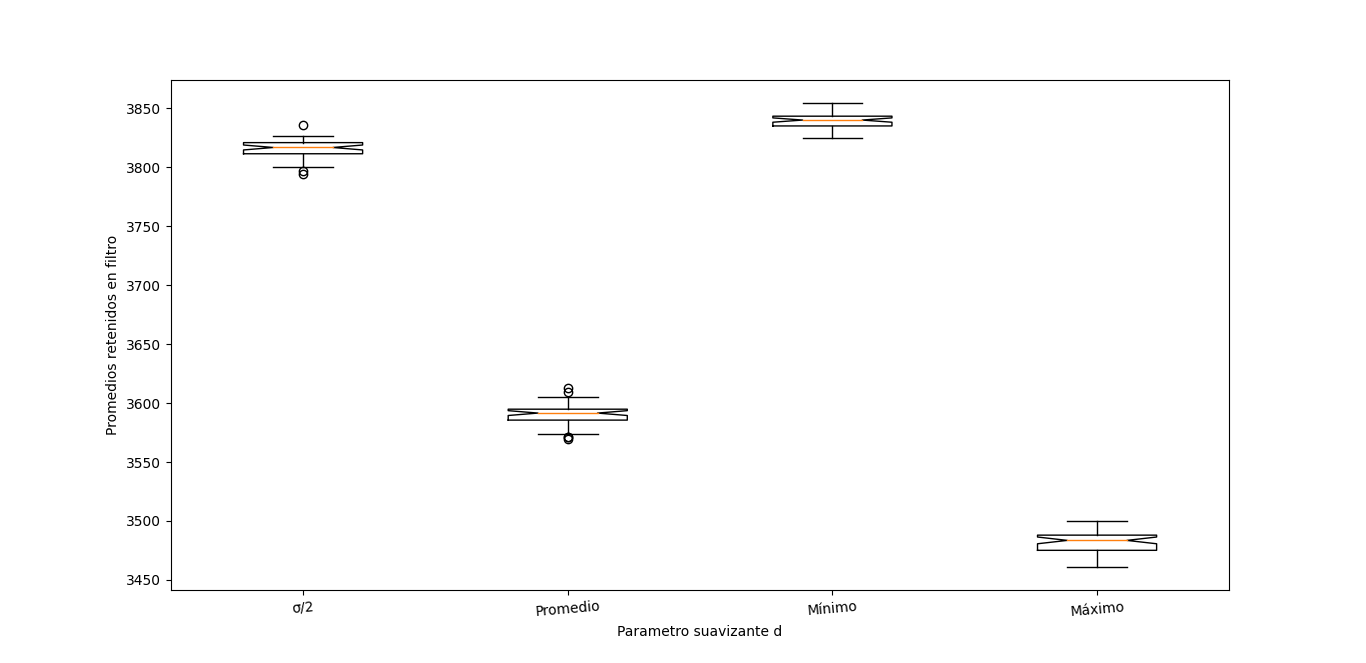
\includegraphics[width=210mm]{Figure_1.1.png}
    \caption{Diagrama de suavizante en $d$.}
    \label{figure}
\end{figure}

\newpage
\bibliographystyle{plainnat}
\bibliography{simulacion}
\end{document}
